%------------------------------------------------------------------------------------------------------------------------
\chapter{シリコンピクセル検出器}
\label{sec:chap2}
%------------------------------------------------------------------------------------------------------------------------
本研究で使用するピクセル検出器は、シリコンを用いた半導体検出器である。本章では、半導体検出器の一般論と、現在ATLAS実験で用いられているピクセル検出器、およびHL-LHCで用いられる新型ピクセル検出器について説明する。

%------------------------------------------------------------------------------------------------------------------------
\section{シリコン検出器}
\label{sec:handoutai}
%------------------------------------------------------------------------------------------------------------------------

%%------------------------------------------------------------------------------------------------------------------------
%\section{半導体検出器の一般論}
%\label{sec:handoutaiippan}
%%------------------------------------------------------------------------------------------------------------------------
本節では,シリコン検出器を例に半導体の主な性質と検出原理について述べる。

%------------------------------------------------------------------------------------------------------------------------
\subsection{半導体検出器の一般論}
\label{sec:handoutai}
%------------------------------------------------------------------------------------------------------------------------
結晶構造を持つ物質は、その電気的な性質から導体、半導体、絶縁体に大別される。半導体は導体と絶縁体の中間程度の電気伝導度を持つ物質であり、この違いはバンドギャップの幅の違いにより説明することができる。結晶構造を持つ物質中では、電子が占有するエネルギー状態はほぼ連続\footnote{電子の存在するエネルギー準位の間隔は$10^{-18}\ [\si{eV}]$と極めて小さいためほぼ連続とみなすことができる。}となり、エネルギーバンドを形成する。
エネルギーバンドの内、フェルミ準位よりエネルギーが高いエネルギー準位を持つものを伝導帯と呼ぶ。伝導帯が電子で満たされていなければ伝導帯に存在する電子は結晶中を自由に移動することができる。また、フェルミ準位より低いエネルギー準位を持つものを価電子帯と呼ぶ。一方で、伝導帯と価電子帯の間の領域を禁制帯と呼ぶ。禁制帯にはエネルギー準位が存在しないため、電子が存在できない。そのため、電子は伝導帯か価電子帯にのみ存在する。
%電子は低い準位から順に占有されるため、価電子帯の準位は充満し、伝導帯には電子が一部のみ存在するかほとんど存在しない。

導体は伝導帯が部分的に電子に占有されているか、伝導体が価電子帯と重なっている状態にある。そのため、伝導帯に存在する電子は、外部電界からエネルギーを受け取り、容易に高い準位に遷移することができる。よって、導体中ではわずかな外部電場により、自由に電子が移動することができる。一方で、半導体や絶縁体では価電子帯の準位は充満し、伝導帯は空となっている。そのため、電流を流すためにはバンドギャップ$E_g$を超えるエネルギーを与え、価電子帯の電子を伝導帯に励起させる必要がある。伝導帯の電子や価電子帯におけるホール(正孔)が結晶中で外部電場により自由に動くことができ、電流が流れる。電子や正孔のような電荷を伝える役割を持つものをキャリアと呼ぶ。半導体ではバンドギャップ$E_g\simeq 1\ \si{eV}$である。$T=0\ \si{K}$では、全ての電子は価電子帯にあり、伝導帯には電子は存在しない。室温$T=300\ \si{K}$ではバンドギャップ$E_g$は熱エネルギー$kT$の数十倍程度であり、わずかな量の電子が価電子帯から伝導帯へ熱的に励起されている。そのため、半導体は低温では絶縁体であり、室温においては電気伝導度が非常に小さい導体のように振る舞う。
絶縁体は$E_g>9\ \si{eV}$と大きなバンドギャップを持つため、伝導帯にいる電子の数は非常に少なく電流は流れない。

%------------------------------------------------------------------------------------------------------------------------
\subsection{n型半導体とp型半導体}
\label{sec:pngata}
%------------------------------------------------------------------------------------------------------------------------
先述したように、半導体は常温で導電性を持つが、導体と比較すると伝導帯に存在する電子は少なく電気伝導度は非常に小さい。電気伝導度を大きくするために半導体に不純物を少量添加する方法により、禁制帯内に新たなバンド構造を作ることができる。これにより、バンドギャップは小さくなり、より多くのキャリアを生成することができ電気伝導度が大きくなる。
%そのため、バンドギャップはさらに小さくなり、電流が流れやすくなる。
添加する不純物の種類により、n型半導体とp型半導体に分類される。

\fref{fig:pgata}にn型半導体の結晶構造とバンド構造を示す。この図は純粋結晶中のシリコン(Si)の1つをリン(P)で置き換えた場合である。4価の元素であるシリコンを5価のリンで置き換えることにより、価電子中の電子が1つ余る。リンと余った電子間の結合エネルギーは、半導体のバンドギャップ$E_g$より小さい。よって、ドナー準位に束縛された電子は、熱エネルギーに容易に伝導帯に励起され、自由電子となる。添加された5価の元素のことをドナーと呼ぶ。
\begin{figure}[tbp]
  \begin{minipage}[b]{0.5\linewidth}
    \centering
    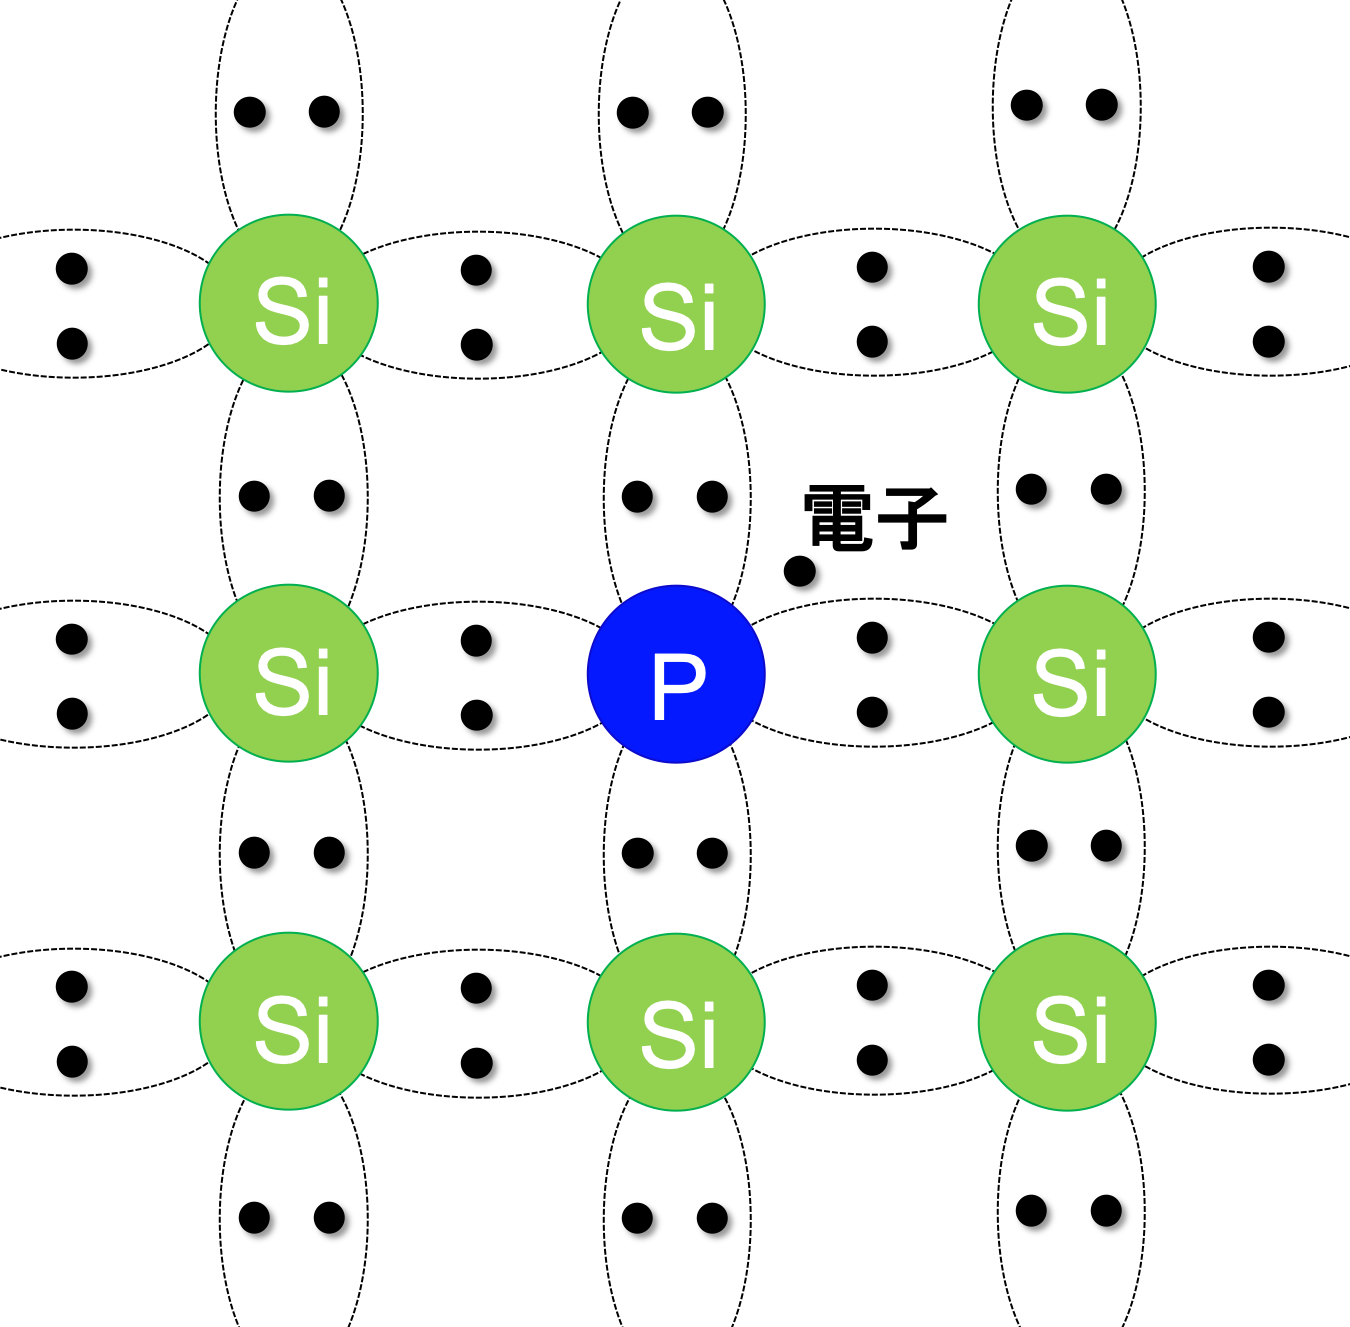
\includegraphics[keepaspectratio, scale=0.25]{ngata1.png}
  \end{minipage}
  \begin{minipage}[b]{0.5\linewidth}
    \centering
    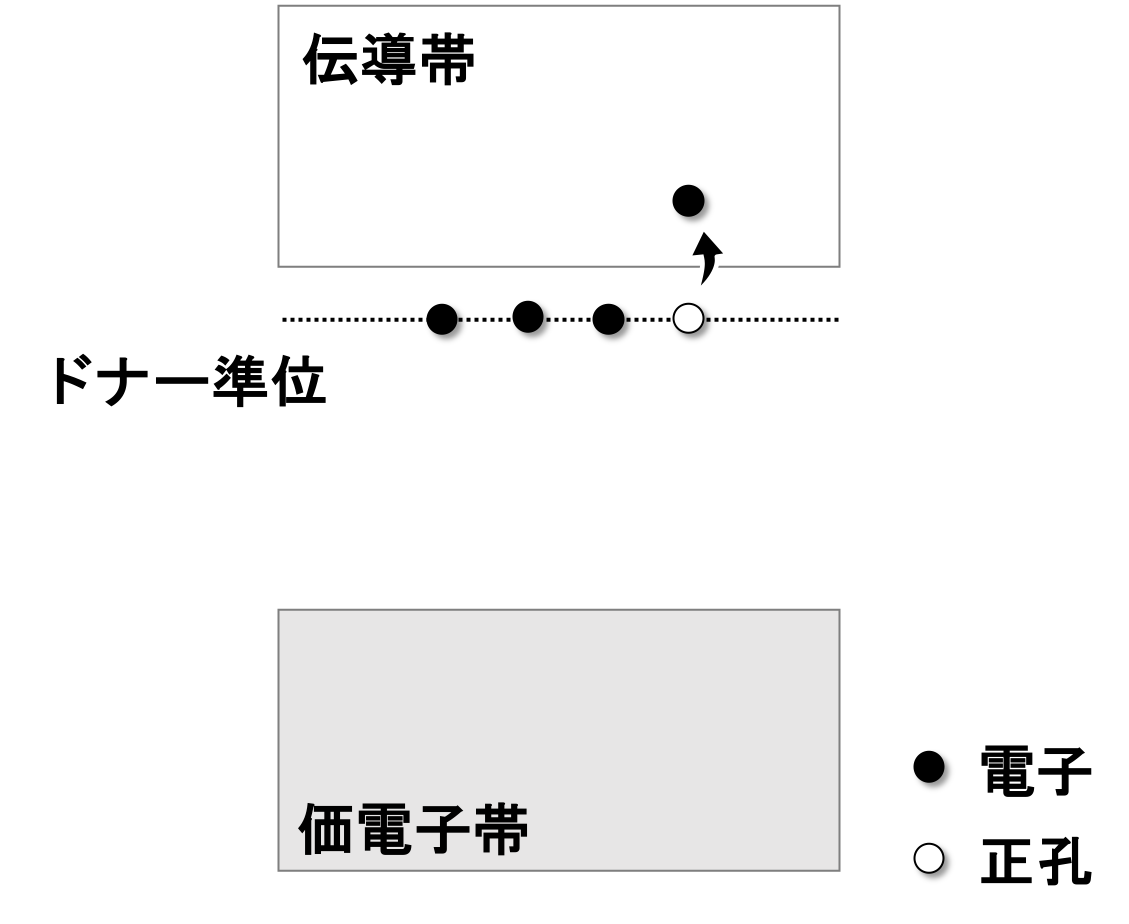
\includegraphics[keepaspectratio, scale=0.3]{ngata2.png}
  \end{minipage}
  \caption[n型半導体の結晶構造とバンド構造]{n型半導体の結晶構造とバンド構造。}
  \label{fig:ngata}
\end{figure}

\fref{fig:pgata}にp型半導体の結晶構造とバンド構造を示す。この図は純粋結晶中のシリコン(Si)の1つをホウ素(B)で置き換えた場合である。4価の元素であるシリコンを3価のホウ素で置き換えることにより、価電子中の電子が不足し正孔が多くなる。これによって得られる正孔の結合エネルギーは、半導体のバンドギャップ$E_g$より小さい。よって、価電子帯の電子は熱的励起により容易にアクセプター準位に励起される。これにより、価電子帯中に1個の自由な正孔が生じて電流を流すことができる。添加された3価の元素のことをアクセプターと呼ぶ。
\begin{figure}[tbp]
  \begin{minipage}[b]{0.45\linewidth}
    \centering
    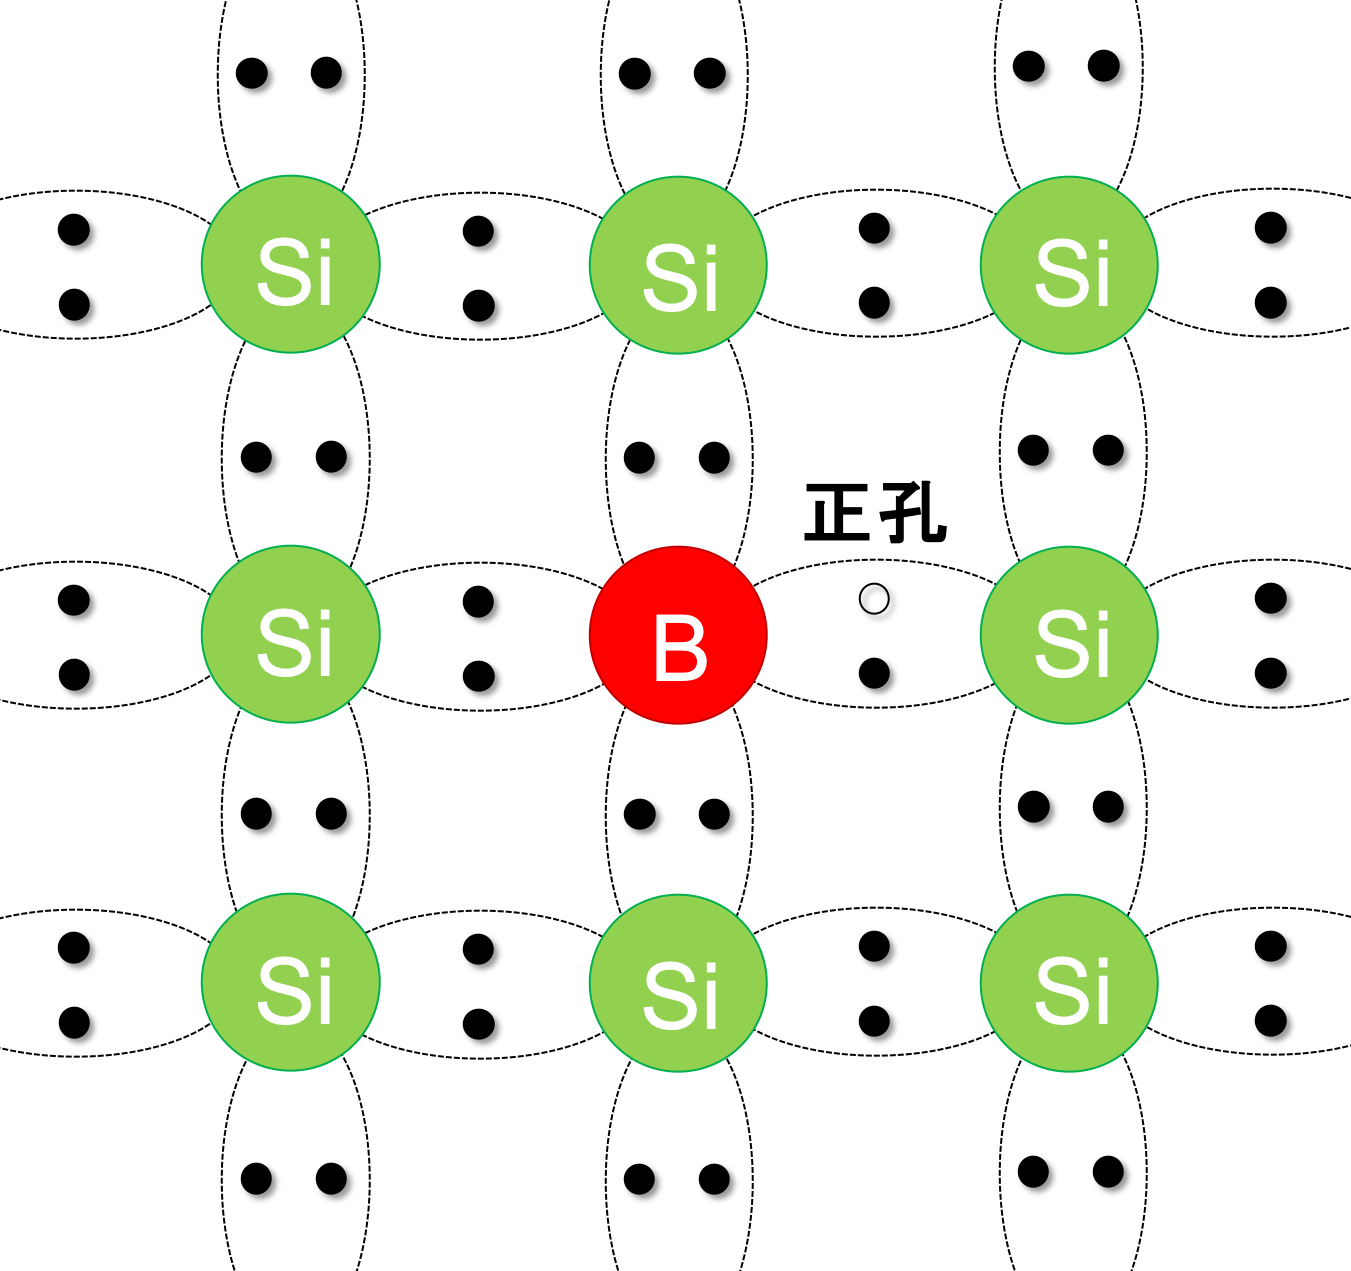
\includegraphics[keepaspectratio, scale=0.25]{pgata1.png}
  \end{minipage}
  \begin{minipage}[b]{0.45\linewidth}
    \centering
    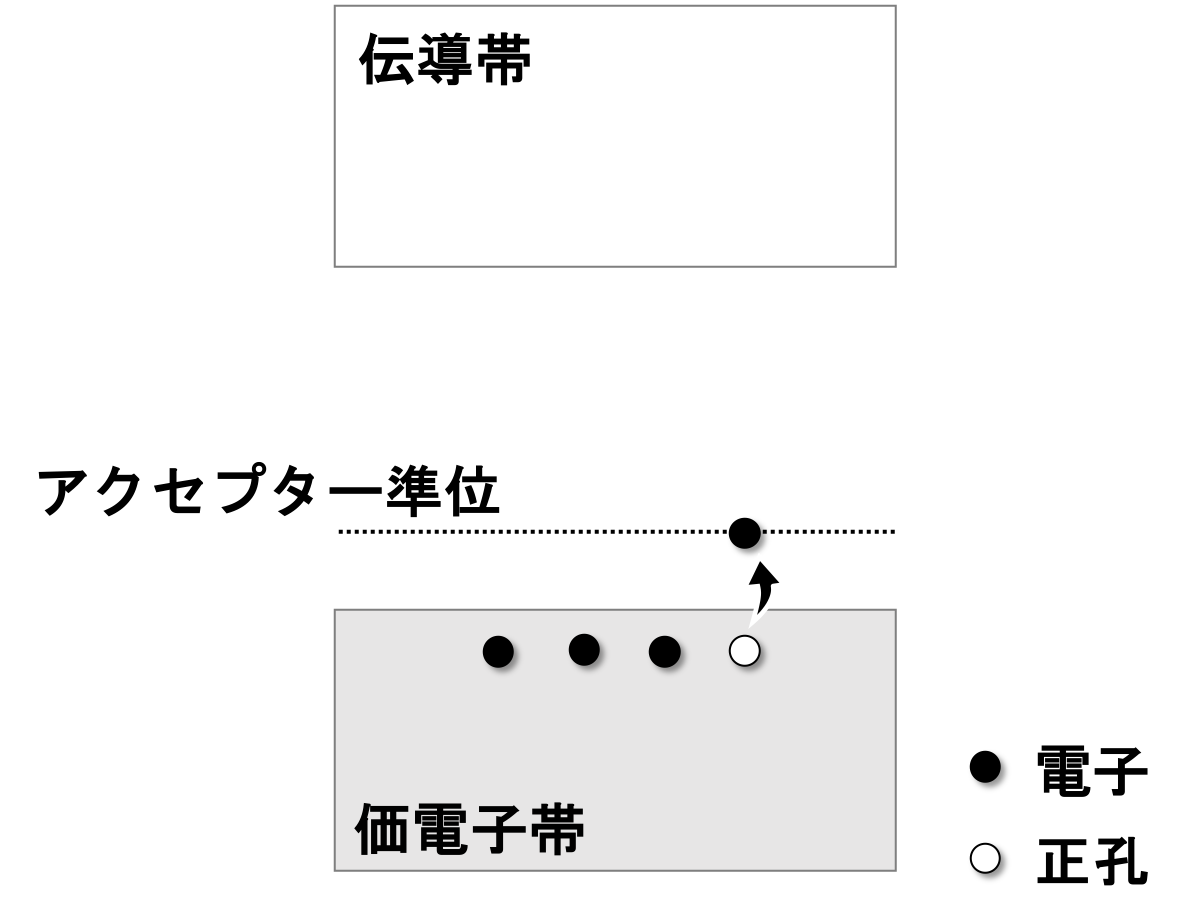
\includegraphics[keepaspectratio, scale=0.3]{pgata2.png}
  \end{minipage}
  \caption[p型半導体の結晶構造とバンド構造]{p型半導体の結晶構造とバンド構造。}
  \label{fig:pgata}
\end{figure}


%------------------------------------------------------------------------------------------------------------------------
\subsection{半導体検出器の動作原理}
\label{sec:pnsetugou}
%------------------------------------------------------------------------------------------------------------------------

半導体検出器は、n型半導体とp型半導体を接合したpn接合を用いて作られる。pn接合の様子を\fref{fig:kuubousou}に示す。pn接合面では、電子と正孔の再結合が起こり、キャリアがほとんど存在しない空乏層と呼ばれる空間が生じる。n型半導体側は電子を失ったことにより正に帯電し、p型半導体側は正孔を失ったことにより負に帯電している。そのため、空乏層の両端に電位差が生じ、これを拡散電位と呼ぶ。空乏層を荷電粒子が通過すると、粒子のエネルギー損失に比例して電子正孔対が生じる。空乏層内で生じた自由な電子や正孔は、拡散電位が作る電場$V_\mathrm{vi}$により電極付近に移動する。これにより、電極表面に電荷が誘起されることで電流が流れることにより信号を生成する。

\begin{figure}[tbp]
  \centering
  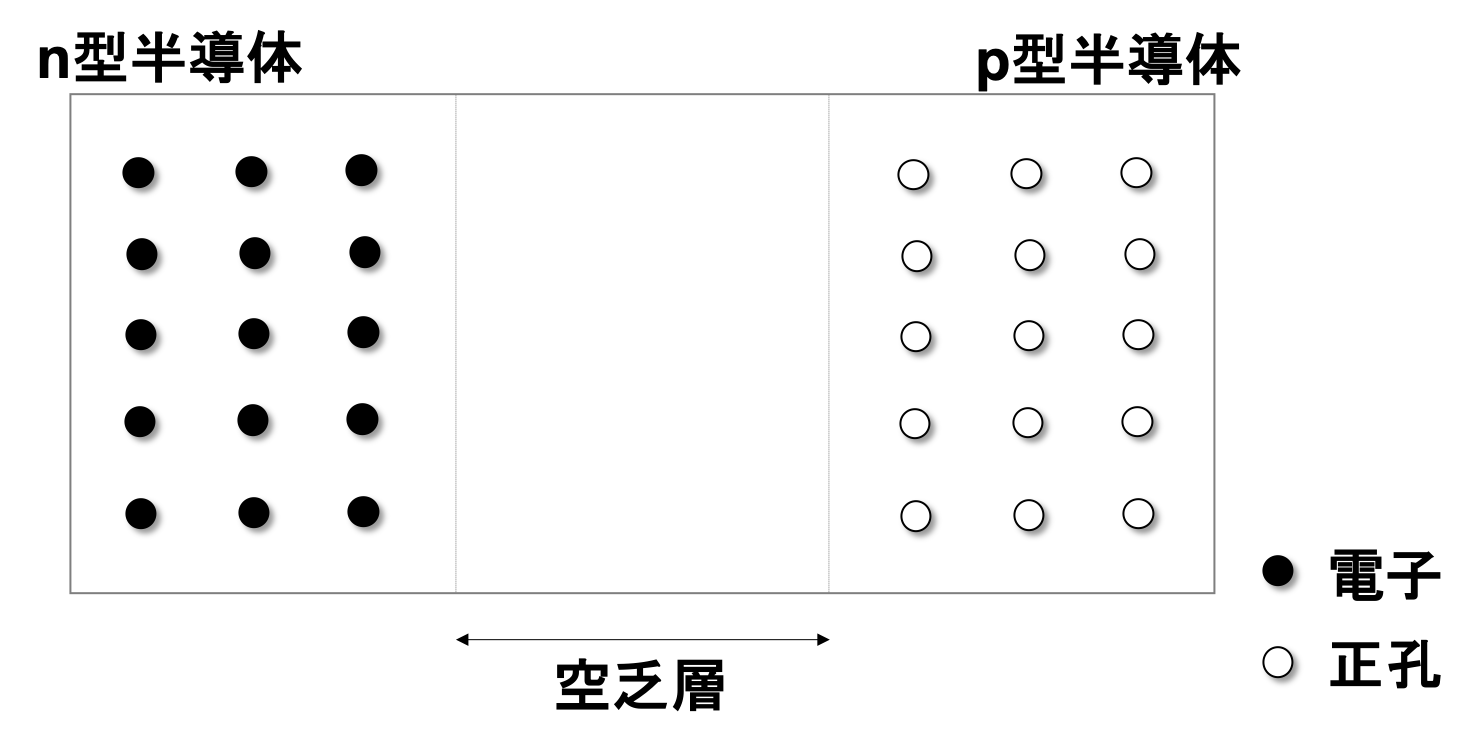
\includegraphics[height=5cm,keepaspectratio]{kuubousou.png}
  \caption[pn接合の様子]{pn接合の様子。}
  \label{fig:kuubousou}
\end{figure}

pn接合から得られる空乏層幅は数$\si{\micro m}$程度である。さらに、拡散電位が作る電場では電荷収集に不十分であり、半導体検出器を飛跡検出器として使用するためにはより大きな電位と広い空乏層幅が必要である。そこで、空乏層幅を広げるために、半導体に外部電場をかける。

空乏層幅$W$とバイアス電圧$V$の関係は\eref{eq:kuubousouhaba}で表される。
\begin{equation}
  \label{eq:kuubousouhaba}
  W = x_n + x_p = \sqrt{\frac{2\varepsilon}{e}\left( \frac{1}{N_A} + \frac{1}{N_D} \right)(V_\mathrm{bi}+V) }
\end{equation}
ここで、$x_n, x_p$はそれぞれn型およびp型半導体中の空乏層の厚さ、$\varepsilon$はシリコンの誘電率、$e$は素電荷、$V_\mathrm{bi}$は拡散電位である。これより、空乏層の幅$W$はバイアス電圧の向きにより変化することがわかる。$V>0$の順バイアス時は空乏層の幅は狭くなり、逆バイアスの時は空乏層の幅が広がる。飛跡検出器としての半導体検出器は、半導体全体を空乏化して使用する。この時、逆バイアス$V$は拡散電位に比べて非常に大きい($V_\mathrm{bi}\ll V$)。さらに、ドナー濃度とアクセプター濃度が同程度のpn接合を用いる場合、\eref{eq:kuubousouhaba}は\eref{eq:kennshutukikuubousou}のように書き直すことができる。
\begin{equation}
  \label{eq:kennshutukikuubousou}
  W \approx \sqrt{\frac{\varepsilon }{eN}V}
\end{equation}
ここで$N$はドナー濃度およびアクセプタ濃度である。このことから、検出器の空乏層幅は逆バイアス電圧の平方根に比例することがわかる。

また、荷電粒子が物質を通過した際のエネルギー損失はBethe-Blochの公式によって記述される。
\begin{equation}
  \label{eq:bethe}
  \left\langle -\frac{dE}{dx} \right\rangle = Kz^2\frac{Z}{A}\frac{1}{\beta^2}\left[ \frac{1}{2}\ln\frac{2m_e c^2 \beta^2 \gamma^2 W_\mathrm{max}}{I^2} -\beta^2 + \frac{\delta (\beta\gamma)}{2} \right]
\end{equation}
ここで、\eref{eq:bethe}における各パラメータは以下の通りである。
\begin{align*}
  \begin{cases}
    dE/dx & \mathrm{単位長さあたりの荷電粒子のエネルギー損失}\ [\si{MeV\cdot g^{-1}\cdot cm^2}]\\
    K & 4\pi N_A r^2_e m_e c^2 = 0.307075\ [\si{MeV\cdot g^{-1}\cdot cm^2}]\ (N_A\mathrm{はアボガドロ定数}, r_e\mathrm{は古典電子半径})\\
    z & \mathrm{荷電粒子の電荷量(素電荷e単位)}\\
    Z & \mathrm{物質の原子番号}\\
    A & \mathrm{物質の原子量}\\
    m_e c^2 & \mathrm{電子の静止エネルギー}(0.511\ [\si{MeV}]) \\
    \beta & \mathrm{荷電粒子の速さと光速の比}\\
    \gamma & \mathrm{ローレンツ因子} 1/\sqrt{1-\beta^2} \\
    W_\mathrm{max} & \mathrm{1度の衝突で物質に与えるエネルギーの最大値} \\
    I & \mathrm{物質の平均励起エネルギー}\\
    \delta & \mathrm{分極による物質の密度補正}
  \end{cases}
\end{align*}
この式から、エネルギー損失$dE/dx$は$\beta$の関数であることがわかる。エネルギー損失$dE/dx$と$\beta$の関係を\fref{fig:bethe}に示す。$\beta$が小さい時は、エネルギー損失は$1/\beta^2$に比例する。$\beta\gamma \simeq 3$あたりで、エネルギー損失は最小値に達する。このエネルギー損失が最小となる粒子をMIP(\textbf{M}inimum \textbf{I}onizing \textbf{P}article)と言う。$\beta\gamma\geq4$からは、$\ln\gamma^2$で緩やかに上昇し、一定値に達する。高エネルギーを持った粒子($\beta\gamma>1$)のエネルギー損失は$1\ \si{MeVg^{-1}cm^2}$と$2\ \si{MeVg^{-1}cm^2}$の間にあることがわかる。薄いシリコンセンサーの場合、検出器内を通過する荷電粒子は制動放射等の放射損失を無視できることができる。そのため、数百$\si{GeV}$のエネルギーを持つ粒子まで同程度のエネルギー損失となり、MIP粒子と見なすことができる。

\begin{figure}[tbp]
  \centering
  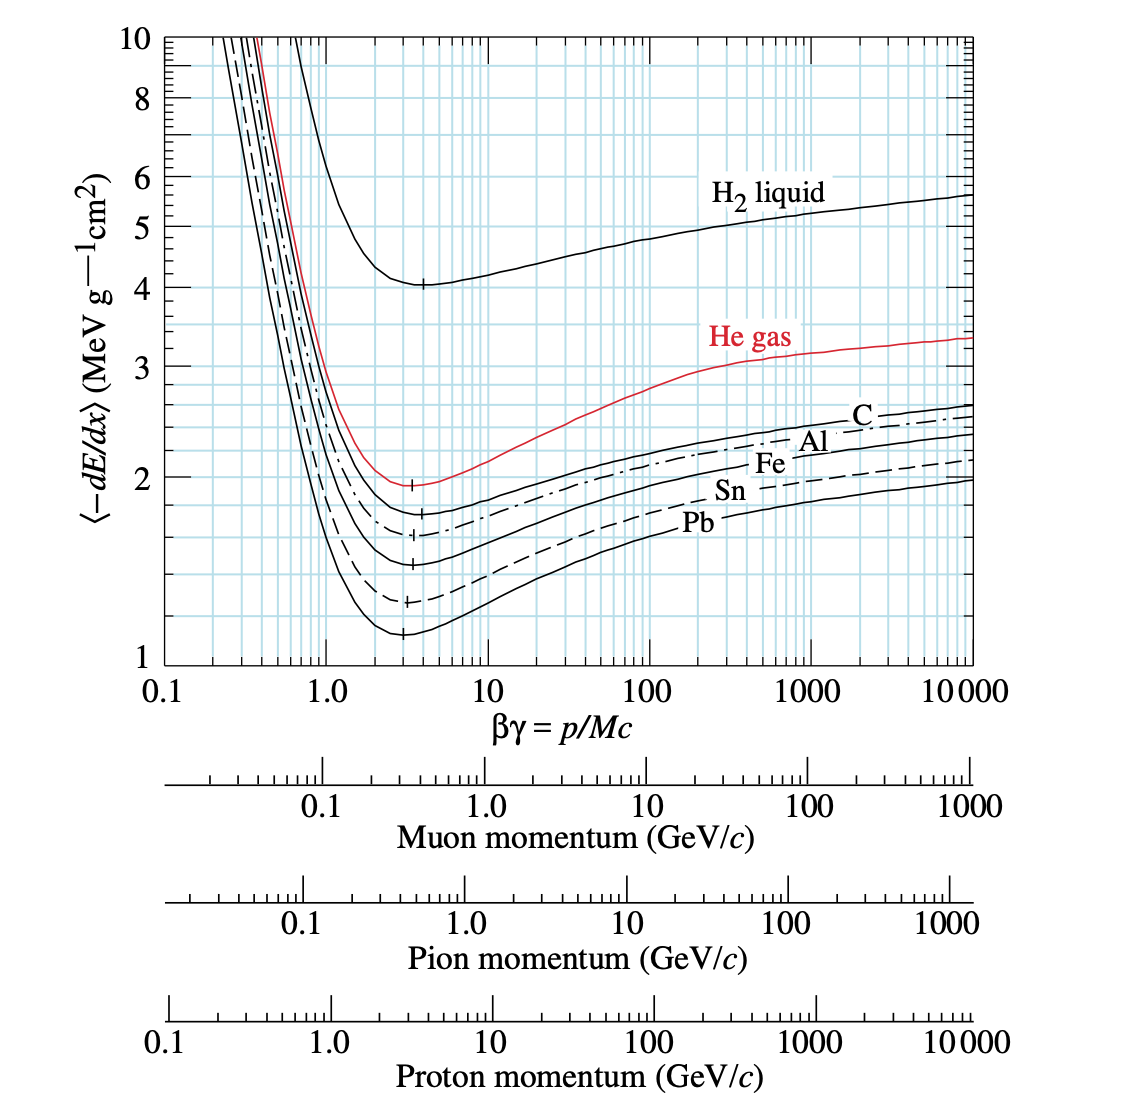
\includegraphics[height=11cm,keepaspectratio]{bethe.png}
  \caption[エネルギー損失と$\beta$の関係。]{エネルギー損失と$\beta$の関係 \cite{bethe}。}
  \label{fig:bethe}
\end{figure}

シリコンの空乏層において、1組の電子正孔対を生成するのに必要なエネルギーは$3.6\ \si{eV}$である。さらに、シリコンの密度は$2.3\ \si{g/cm^3}$であるため、高エネルギー粒子がシリコン内に通過した時に単位距離当たりに生成される電子正孔対は約$50\ \si{e / \micro m}$となる。
%\begin{equation}
%  \label{eq:tanniseikou}
%  1\ \si{MeVg^{-1}cm^2} \times 2.3\ \si{g/cm^3} / (3.6\ \si{eV})\approx 60\ \si{\micro m^{-1}}
%\end{equation}


%------------------------------------------------------------------------------------------------------------------------
\section{ピクセルモジュール}
\label{sec:pixelkenshutuki}
%------------------------------------------------------------------------------------------------------------------------

ATLASのシリコンピクセル検出器は、\textbf{ピクセルモジュール}と呼ばれる最小単位の\fref{fig:pikuserukennshutuki}にピクセルモジュールの模式図を示す。ピクセルモジュールはシリコンセンサー、FE(\textbf{F}ront-\textbf{e}nd)チップ、フレキシブル基板から構成される。この節ではそれぞれについて説明する。

\begin{figure}[tbp]
  \centering
  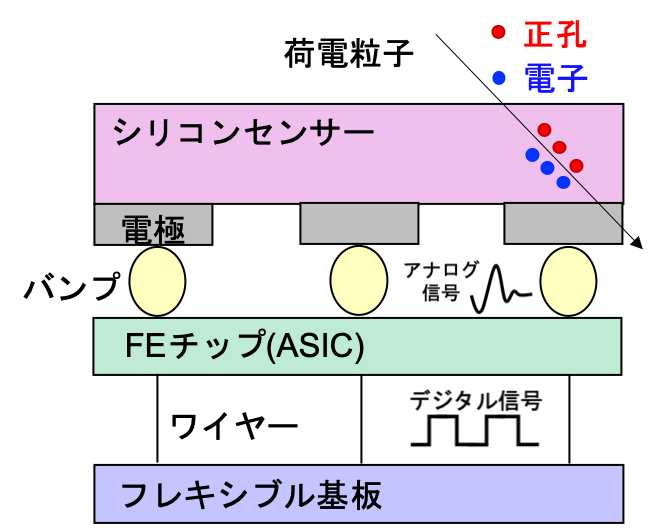
\includegraphics[height=7cm,keepaspectratio]{pikuserukennshutuki.png}
  \caption[ピクセルモジュールの模式図]{ピクセルモジュールの模式図。}
  \label{fig:pikuserukennshutuki}
\end{figure}

%------------------------------------------------------------------------------------------------------------------------
\subsection{シリコンセンサー}
\label{sec:silicon}
%------------------------------------------------------------------------------------------------------------------------
ATLASピクセル検出器に実装するセンサーはプラナーセンサーと3Dセンサーがある。\fref{fig:3dplanar}にプラナーセンサーと3センサーの模式図を示す。

プラナーセンサーは、\fref{fig:3dplanar}の左のようにセンサーのバルク部の表面にn$^+$型半導体と$p^+$型半導体を埋め込んだ構造をしている。$n^+$型半導体電極はセンサー面において格子状に配列し、それぞれの電極から独立した信号を読み出すことができる。IBLおよびピクセル検出器ではバルク部にn型半導体を用いた、n$^{+}$-in-n型と呼ばれるものを用いている。n$^{+}$-in-n型の場合、空乏層はp$^{+}$型インプラントとn型バルクの境界から成長する。そのため、荷電粒子が空乏層を通過した際に信号をn$^{+}$電極において検知するためには、空乏領域をn$^{+}$電極まで広げる必要があり、完全空乏化しなければならない。さらに、バルク部のn型半導体は放射線損傷によりp型に型変換を起こし、空乏化の挙動が変化する。HL-LHCでは放射線損傷の影響がより大きくなることが想定されているため、センサーの挙動変化をさせないために、ITkではn$^{+}$-in-p型のセンサーを用いる。n$^{+}$-in-p型の場合、空乏領域がn$^{+}$電極とp型バルクの境界から空乏領域が成長するため、完全空乏化しなくても荷電粒子の通過により生じる電子を検知することができる。p型半導体は放射線損傷により完全空乏化電圧が大きくなるためより大きな電圧が必要になるが、全空乏化電圧が耐電圧を超えたら部分空乏化による運用が可能である。


3Dセンサーはセンサー面に対して垂直に柱状の電極インプラントをしたものである。3Dセンサーは電極間の距離が短いことから、全空乏化に必要な電圧が小さい。さらに生成した電子正孔対が電極に到達するまでの距離も短いため、格子欠損により生じたホールにトラップされる確率もプラナーセンサーに比べて小さい。そのため、3Dセンサーはプラナーセンサーに比べて放射線耐性の高いセンサーである。3Dセンサーは放射線損傷の影響が大きいIBLの一部のみに実装されており、ITkの一部にも搭載する予定である。

\begin{figure}[tbp]
  \begin{minipage}[b]{0.45\linewidth}
    \centering
    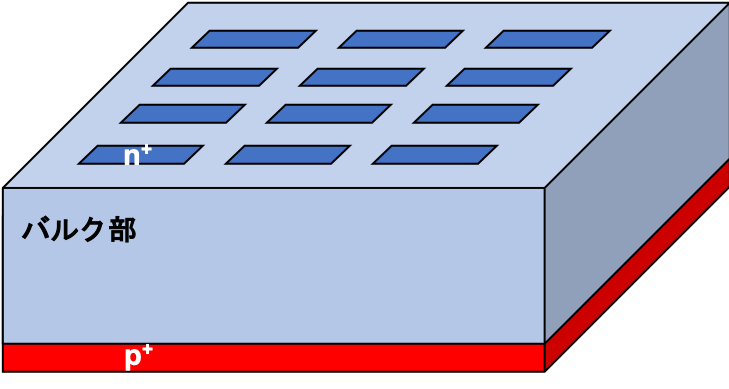
\includegraphics[keepaspectratio, scale=0.5]{planar.png}
  \end{minipage}
  \begin{minipage}[b]{0.45\linewidth}
    \centering
    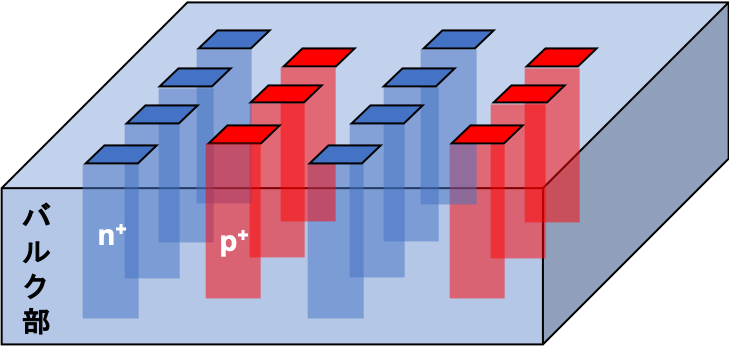
\includegraphics[keepaspectratio, scale=0.55]{3dsensor.png}
  \end{minipage}
  \caption[プラナーセンサーと3Dセンサーの構造]{プラナーセンサー(左図)と3Dセンサーの構造(右図)。}
  \label{fig:3dplanar}
\end{figure}


%------------------------------------------------------------------------------------------------------------------------
\subsection{FEチップ}
\label{sec:ASIC}
%------------------------------------------------------------------------------------------------------------------------

FEチップは特定用途向けに複数機能を実装した集積回路(ASIC: \textbf{A}pplication \textbf{S}pecific \textbf{I}ntegrated \textbf{C}ircuit)である。センサーの電極で収集された電荷は、バンプを通ってFEチップに送られる。FEチップでは受け取ったアナログ信号を増幅、整形、デジタル処理を行い後段の読み出し基板に信号を送る。
%\begin{figure}[tbp]
%  \centering
%  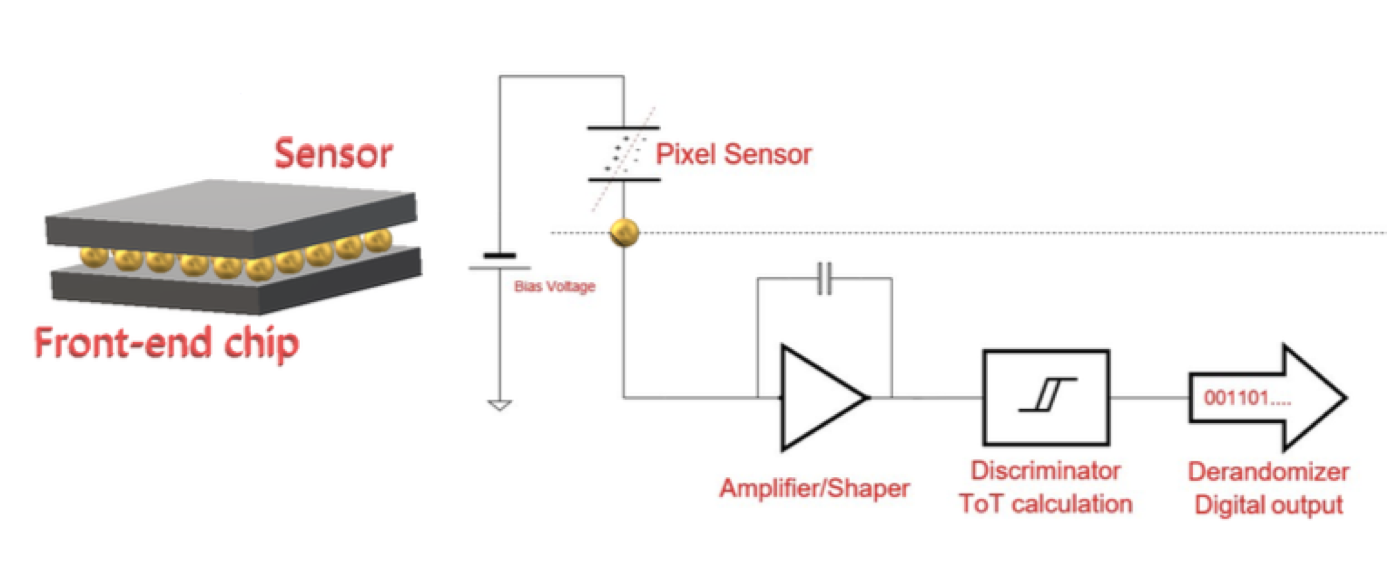
\includegraphics[height=6cm,keepaspectratio]{asic.png}
%  \caption[シリコンセンサーの模式図]{シリコンセンサーの模式図。}
%  \label{fig:asic}
%\end{figure}

センサーを通過する荷電粒子は、電子正孔対を生成する。シリコンの空乏層で1組の電子正孔対を生成するのに必要なエネルギーは$3.6\ \si{eV}$と一定のため、生成される電子正孔対の数はエネルギー損失$dE/dx$に比例する。
生成されたキャリアが電極付近に収集され、電極の内部電位に影響を与えて電流が流れる。この電流から得られるアナログ信号をFEチップにおいて増幅、整形を行う。アナログ信号はアンプ回路により増幅され、三角波になるよう波形整形が行われる。信号処理されたアナログ信号がThresholdを超えた時間幅を測定し、デジタル信号に変換する。このデジタル信号を\textbf{Time over Threshold} (\textbf{ToT})と呼ぶ。アナログ信号をToTに変換する概念図を\fref{fig:tot}に示す。時間幅は$25\ \si{ns}$間隔のクロックの数で取得するため、デジタル信号として取得することができ、この信号が後段のフレキシブル基板へ転送される。

\begin{figure}[tbp]
  \centering
  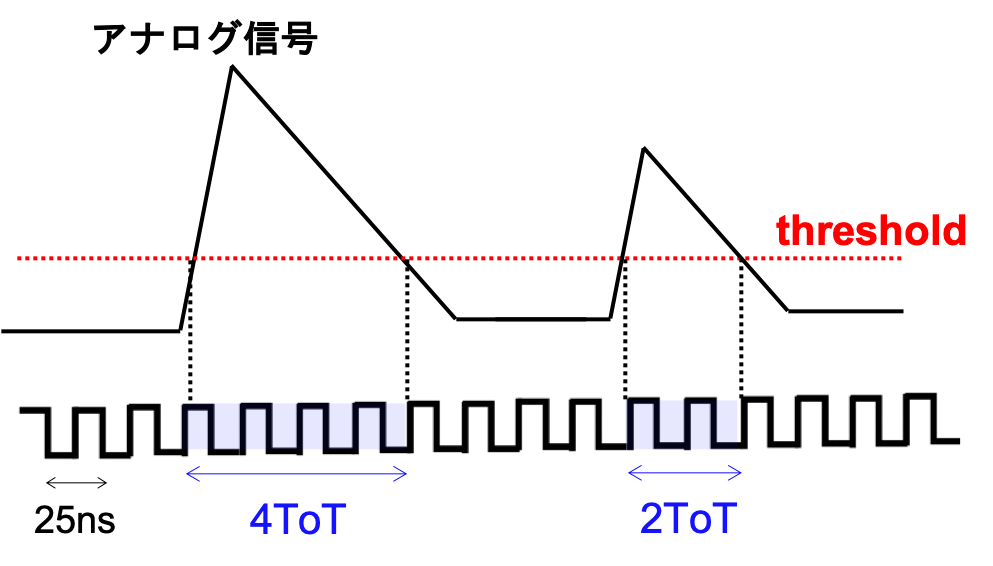
\includegraphics[height=5cm,keepaspectratio]{tot.png}
  \caption[アナログ信号をToTに変換する概念図]{アナログ信号をToTに変換する概念図。アナログ信号の三角波はThresholdを超えた時間幅に相当する量であるToTに変換される。}
  \label{fig:tot}
\end{figure}

また、アナログ回路により信号の立ち上がりから三角波の頂点までにかかる時間は、電荷量に依存せず約$40\ \si{ns}$となるよう設定されている。そのため、小さい電荷量から生成される信号は立ち上がりが遅くなってしまう。時間幅は$25\ \si{ns}$を単位とするクロックで測定されるが、クロックの間隔が$25\ \si{ns}$と短いため、アナログ信号のパルスの立ち上がりからThresholdを超えるまでの時間である\textbf{タイムウォーク}の効果を考慮する必要がある。電荷量とタイムウォークの関係を\fref{fig:timewalk}に示す。電荷量の小さい信号は、タイムウォークの影響が大きくなり、本来とは異なる位置からToTの測定を開始してしまう恐れがある。ATLASにおける陽子衝突は$40\ \si{MHz}$で起きているため、タイムウォークの影響が大きくなるものは異なる物理事象と関連付けてしまう可能性がある。そこで、このような影響を抑えるために、\textbf{Intime threshold}という新たな閾値を導入する。Intime thresholdは、$100\ \si{ke}$を持つ参照電荷と比べてタイムウォークが$20\ \si{ns}$長くなるアナログ信号の電荷量として定義される。そのため、Intime thresholdはThresholdよりも大きい値(おおよそThresholdの値よりも$1500\ \si{e}$程度大きい値)になるよう決定され、タイムウォークの影響の制御をすることができる。


%\begin{figure}[tbp]
%  \begin{minipage}[b]{0.5\linewidth}
%    \centering
%    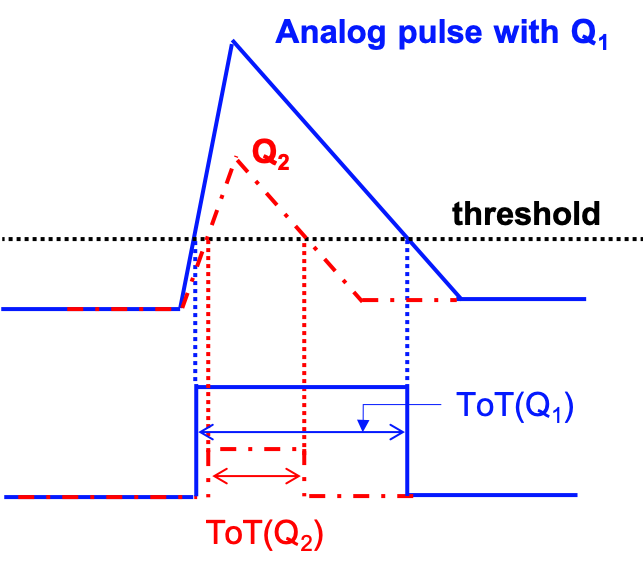
\includegraphics[keepaspectratio, scale=0.6]{calibeq2.png}
%  \end{minipage}
%  \begin{minipage}[b]{0.5\linewidth}
%    \centering
%    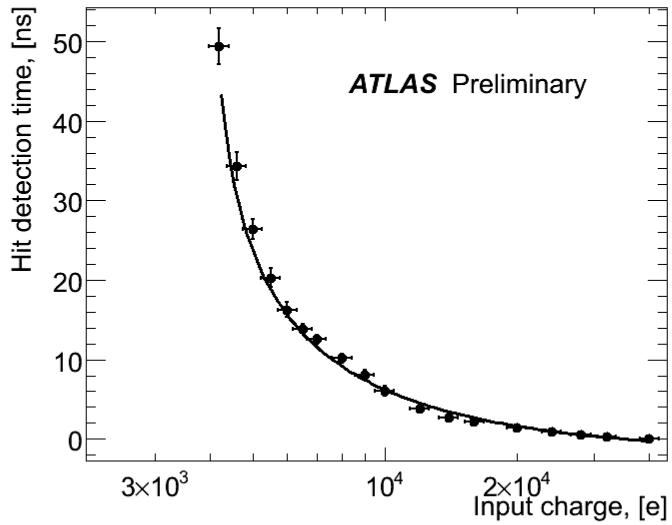
\includegraphics[keepaspectratio, scale=0.6]{timewalk.png}
%  \end{minipage}
%  \caption[ToTと荷電粒子がシリコンセンサーに落とす電荷量$Q$の概念図]{ToTと荷電粒子がシリコンセンサーに落とす電荷量$Q$の概念図。図中の青線と赤線はある電荷量$(Q_1>Q_2)$がToTに変換される概念図である。左図はToTと電荷量$Q$の関係が理想的に線形になる場合で、右図はタイムウォーク等の二次的な効果を受けた場合の図である。図中上半分の三角波はアナログ回路のフィードバック回路にて整形・増幅された信号であり、その信号がThreshold値を超える時間であるToTに変換される。三角波の立ち上がりはタイムウォークによって変化するが、立ち下がりはフィードバック回路によって制御されるため、電荷量に依存せず一定の傾きである。}
%  \label{fig:calibnijikouka}
%\end{figure}

\begin{figure}[tbp]
  \centering
  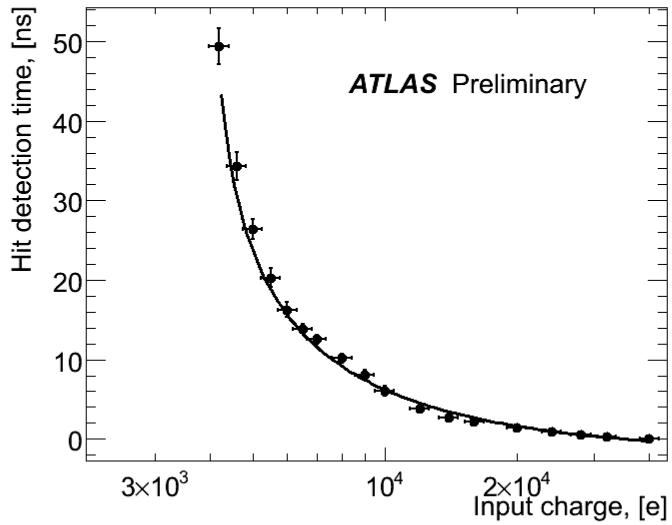
\includegraphics[height=6cm,keepaspectratio]{timewalk.png}
  \caption[電荷量とタイムウォークの関係]{電荷量とタイムウォークの関係 \cite{timewalk}。}
  \label{fig:timewalk}
\end{figure}


ピクセル検出器では\textbf{FE-I3}というFEチップを用いている。さらに読み出し速度等の性能を向上させたものが、IBLに用いられている\textbf{FE-I4}である。また、HL-LHCアップグレードに向けて新たなFEチップの開発が進んでいる。ITkに搭載する新型FEチップはITk pix v2と呼ばれており、プロトタイプであるRD53AおよびITk pix v1の製作が進んでいる。
それぞれのFEチップの主な仕様の比較を\tref{tab:asicsiyou}に示す。

\begin{table}[tbp]
  \begin{center}
    \caption[各FEチップの主な仕様]{各FEチップの主な仕様 \cite{itk}。}
    \label{tab:asicsiyou}
    \begin{tabular}{|c||c|c|c|}
    \hline
      項目 & FE-I3 & FE-I4 & ITk pix v2 \\
    \bhline{1.5pt}
      チップサイズ$[\si{mm^2}]$ & $7.6\times10.8$ & $20.2\times 19.0$ & $20.0\times 20.0$ \\
    \hline
      ピクセルサイズ$[\si{\micro m^2}]$ & $50\times 400$ & $50\times 250$ & $50\times 50$ \\
    \hline
      ピクセル数 & $18\times160$ & $80\times336$ & $400\times 384$ \\
    \hline
      データ転送速度$[\si{Mbps}]$ & $40$ & $160$ & $1280\times 4$ \\
    \hline
      トリガーレート$[\si{kHz}]$ & $100$ & $300$ & $1000$ \\
    \hline
    \end{tabular}
  \end{center}
\end{table}

RD53AはATLASおよびCMS\footnote{CMSはLHC上の4つの衝突点の1つで行われている実験である。}が共同で開発を進めているHL-LHCのための試作器であり、試験・比較のために3種類のアナログ回路を搭載している。\fref{fig:rd53a}にRD53Aのを示す。\fref{fig:rd53a}のようにRD53Aには3つの領域があり、左から順にSynchronous FE、Linear FE、Differrential FEと呼ぶ。それぞれの領域においてアナログ信号の処理方法が異なり、Differential FEは他のFEと比較して電気ノイズが低くなることがわかっている。そのため、ITkにはDifferential FEを用いることが決定している。

\begin{figure}[tbp]
  \centering
  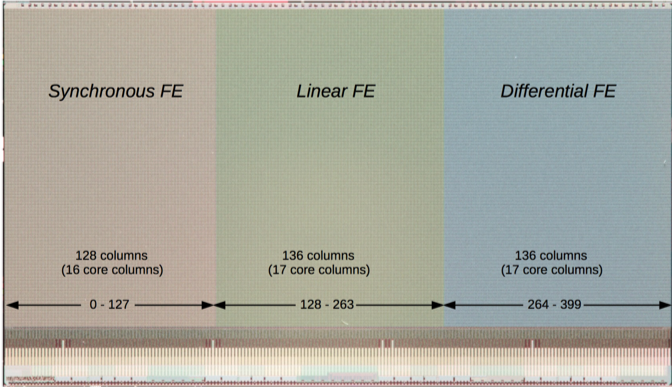
\includegraphics[height=5cm,keepaspectratio]{rd53a.png}
  \caption[RD53Aのピクセルとアナログ回路]{RD53Aのピクセルとアナログ回路\cite{rd53a}。左の領域から順にSynchronous FE、Linear FE、Differrential FEとなっている。}
  \label{fig:rd53a}
\end{figure}

ITk pix v1は、外形形状と主な仕様についてITkに搭載されるFEチップと同様の構造を持つ試作器である。ITk pix v1の段階で発見された不具合やバグ等を修正し量産するものが、ITkに搭載するFEチップの\textbf{ITk pix v2}である。



%------------------------------------------------------------------------------------------------------------------------
\section{放射線損傷}
\label{sec:houshasennsonnshou}
%------------------------------------------------------------------------------------------------------------------------
ATLAS実験において、シリコンピクセル検出器は、ビーム衝突点のすぐ近くに配置される。そのため、陽子衝突から生成される多数の粒子が検出器中を通過するため、検出器は放射線による損傷を受ける。高放射線環境下で起こる典型的な放射線損傷はバルク損傷と表面損傷の2つに大別される。この節ではそれらについて説明する。


%------------------------------------------------------------------------------------------------------------------------
\subsection{バルク損傷}
\label{sec:baruku}
%------------------------------------------------------------------------------------------------------------------------
バルク損傷とは、放射線が結晶中のシリコン原子と相互作用し、原子が結晶位置から弾き出される現象である。弾き出された原子が格子間に原子となり、格子点ではない場所に入り込むものをフレンケル欠陥と呼ぶ。また、弾き出された原子が格子点を離れて結晶表面に移動し、結晶内に空孔のみが存在してできる欠陥をショットキー欠陥と呼ぶ。
\begin{figure}[tbp]
  \begin{minipage}[b]{0.45\linewidth}
    \centering
    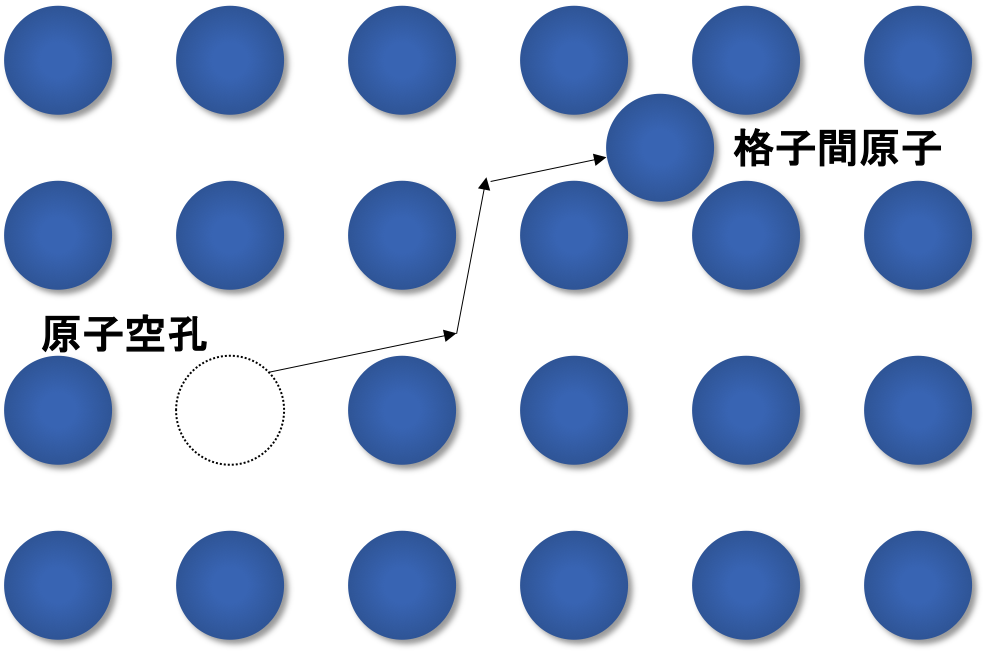
\includegraphics[keepaspectratio, scale=0.3]{flenkel.png}
  \end{minipage}
  \begin{minipage}[b]{0.45\linewidth}
    \centering
    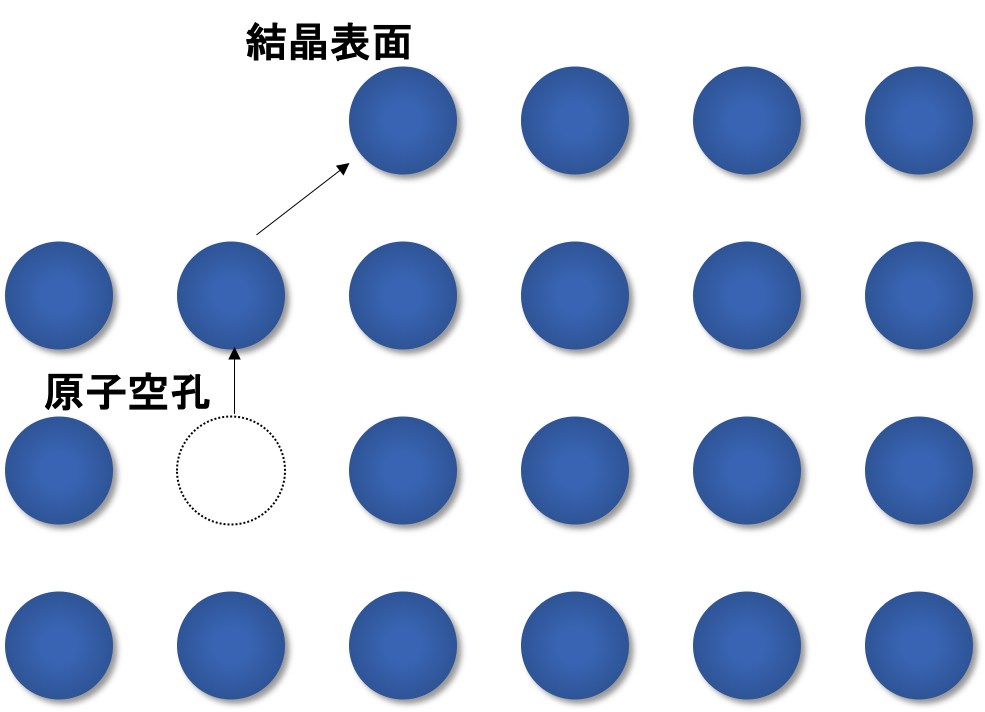
\includegraphics[keepaspectratio, scale=0.3]{shotkey.png}
  \end{minipage}
  \caption[フレンケル欠陥とショットキー欠陥]{フレンケル欠陥(左図)とショットキー欠陥(右図)。図中における青丸は原子核を表す。}
  \label{fig:kekkan}
\end{figure}


フレンケル欠陥とショットキー欠陥はどちらも原子核欠損のため、実行的にはp型不純物として働く。これにより、検出器に以下のような影響を及ぼす。
\begin{itemize}
  \item 暗電流の増加\\
  格子欠陥はp型不純物として働くため、バンドギャップ内に新たなエネルギー準位を作る。この準位が自由な正孔を作るため、暗電流が流れる。この電流はバルクが浴びる放射線量に比例して増加する。
  \item バルクの型変換と全空乏化電圧の増加\\
  格子欠陥はp型不純物として働くため、アクセプター濃度$N_A$が増加させる。n型半導体に格子欠陥が生じると実効的なドナー濃度$N_D$が低下し、やがてアクセプター濃度が損傷前のドナー濃度より大きくなり、p型半導体のように振る舞う。これを半導体の型変換という。また、p型半導体に格子欠陥が生じると、実効的なアクセプター濃度$N_A$が増大し、全空乏化電圧が大きくなる。放射線損傷による型変換および全空乏化電圧の測定結果を\fref{fig:katahennkann}に示す。
\end{itemize}
\begin{figure}[tbp]
  \centering
  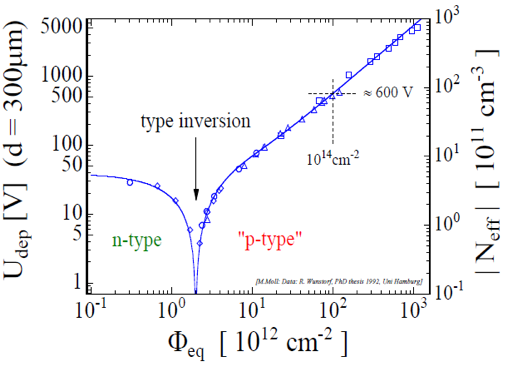
\includegraphics[height=7cm,keepaspectratio]{katahennkann.png}
  \caption[放射線損傷による型変換および全空乏化電圧の測定結果]{n型シリコン検出器を用いた放射線損傷による型変換および全空乏化電圧の測定結果\cite{typeinversion}。}
  \label{fig:katahennkann}
\end{figure}



%------------------------------------------------------------------------------------------------------------------------
\subsection{表面損傷}
\label{sec:hyoumen}
%------------------------------------------------------------------------------------------------------------------------
表面損傷は、シリコンセンサーの表面を覆う誘電体等が受ける放射線損傷の総称であり、主に$300\ \si{keV}$以下のエネルギーを持つ光子や荷電粒子によって生じる。表面を覆うSiO$_2$層を荷電粒子が通過し、電子正孔対が生成される。電子正孔対は大部分は再結合するが、SiO$_2$内での正孔の移動度は電子の移動度に比べて非常に小さいため、捕獲できなかった電子は読み出し電極に収集される。この正孔がSi-SiO$_2$界面に集まり、正の電場を作ることにより、この電場に電子が引きつけられて電荷収集効率が低下する。


%------------------------------------------------------------------------------------------------------------------------
\subsubsection{表面損傷とトータルドーズ効果}
\label{sec:totaldoze}
%------------------------------------------------------------------------------------------------------------------------

ATLASのFEチップには、回路内にMOSトランジスタが使用されている。MOSトランジスタの模式図を\fref{fig:mos}に示す。MOSトランジスタは、ゲートに電圧をかけることにより電荷が誘起され、ソースとドレイン間に電流が流れる仕組みになっている。MOSトランジスタはSTIと呼ばれる酸化膜により周囲と絶縁している。しかし、トータルドーズ効果と呼ばれる放射線損傷により、酸化膜がイオン化し、その結果正孔が酸化膜界面に収集される事により、\fref{fig:mos}の右図の黄色の領域が正に帯電する。それにより、シリコン内に負の電荷が誘起され、本来絶縁されているはずのソース・ドレイン間に電流が流れやすくなる。

\begin{figure}[tbp]
  \begin{minipage}[b]{0.5\linewidth}
    \centering
    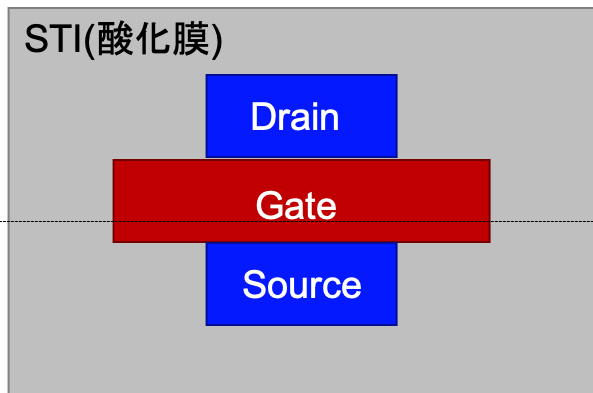
\includegraphics[keepaspectratio, scale=0.5]{mos1.png}
  \end{minipage}
  \begin{minipage}[b]{0.5\linewidth}
    \centering
    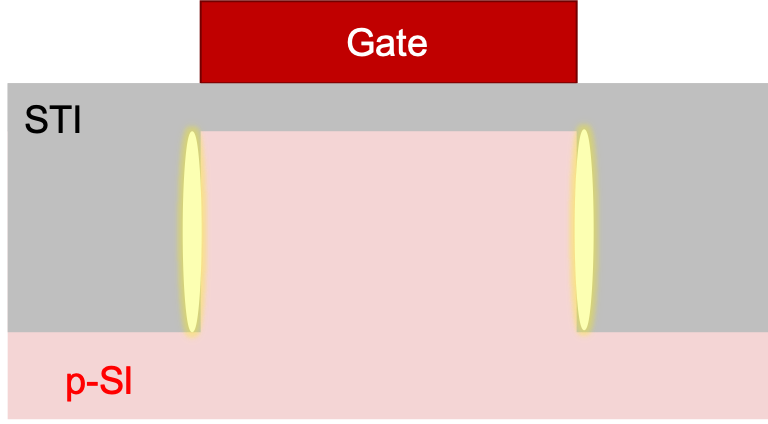
\includegraphics[keepaspectratio, scale=0.45]{mos2.png}
  \end{minipage}
  \caption[MOSトランジスタの模式図]{MOSトランジスタの模式図。左図の点線部の断面図が右図に相当する。}
  \label{fig:mos}
\end{figure}

トータルドーズ効果(TID: \textbf{T}otal \textbf{I}onizing \textbf{D}ose)とは、多量の放射線による電離作用によって引き起こされる。半導体内の電離作用によって生じた正孔が表面の酸化膜にトラップされるなど、半導体の特性に影響を与える効果である。
トータルドーズ効果とFEチップ電流の関係を\fref{fig:totaldoze}示す。

\begin{figure}[tbp]
  \centering
  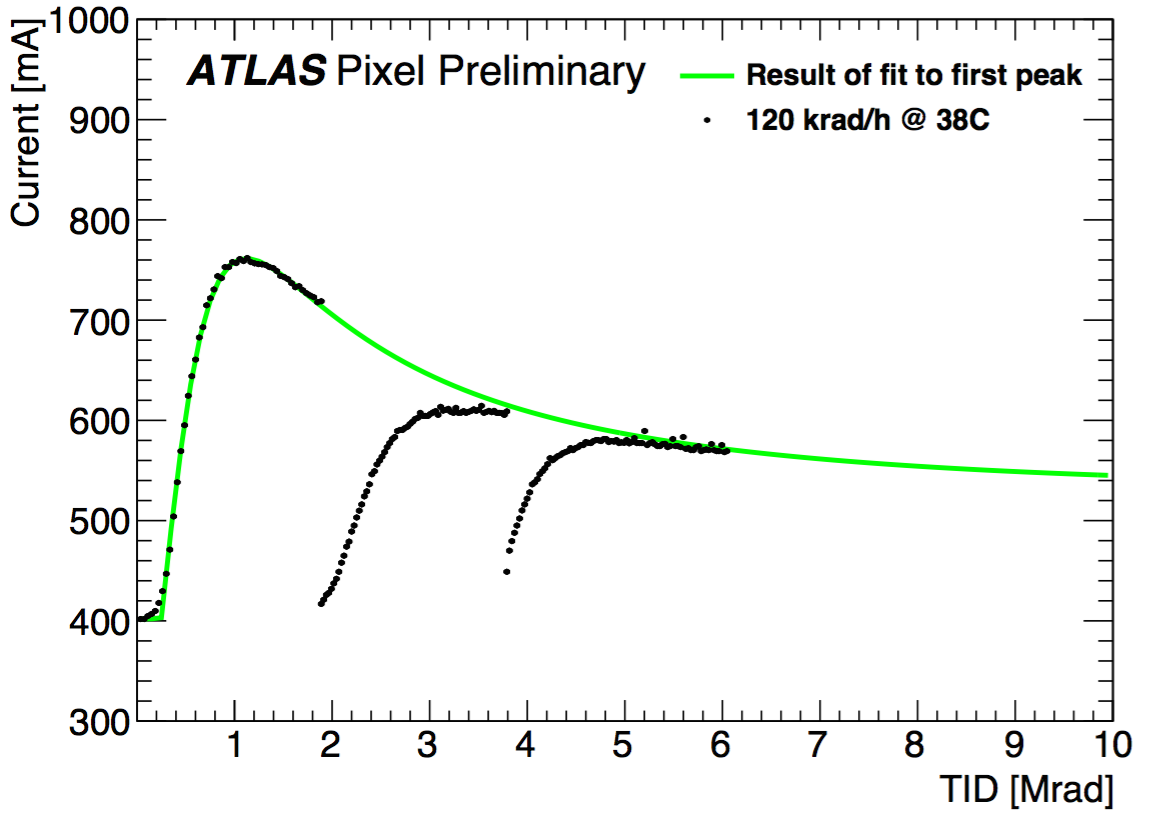
\includegraphics[height=7.5cm,keepaspectratio]{totaldose.png}
  \caption[トータルドーズ効果とFEチップ電流の関係]{トータルドーズ効果とFEチップ電流の関係 \cite{tid}。FEチップの周囲温度$38\ \si{\degreeCelsius}$および単位時間あたりの放射線量$120\ \si{krad}$での測定結果である。緑線は最初のピークに対するフィッティング結果である。また、各ピークが最大になった後、FEチップを数時間アニールする事により、部分的に放射線損傷が回復していることがわかる。}
  \label{fig:totaldoze}
\end{figure}

放射線損傷が少ない場合(TID $\lesssim 1\ [\si{Mrad}]$)、トータルドーズ効果によって生じた正孔は、Si-SiO$_{2}$界面に収集され電場を形成する。その電場に電子が引きつけられる事により、本来絶縁されているソース・ドレイン間に電流が流れやすくなってしまう。その結果、FEチップに流れる電流が増加し、回路内のアンプやディスクリミネータなどあらゆる回路の挙動に影響を与える。\fref{fig:tidhennka}にトータルドーズ効果とThresholdおよびToTの関係を示す。この図から、放射量が増えるとThresholdは大きくなり、ToTの値は小さくなることがわかる。

一方で、放射線損傷が大きくなる(TID $\gtrsim 1\ [\si{Mrad}]$)と、正孔付近にも電子が捕獲されるようになり、Si-SiO$_{2}$界面に収集された正孔による電場が徐々に小さくなる。そのため、リーク電流が小さくなり、ThresholdおよびToTの値が変化する。この場合については、放射量が増加するとThresholdは小さくなり、ToTは大きくなる。

\begin{figure}[tbp]
  \begin{minipage}[b]{0.5\linewidth}
    \centering
    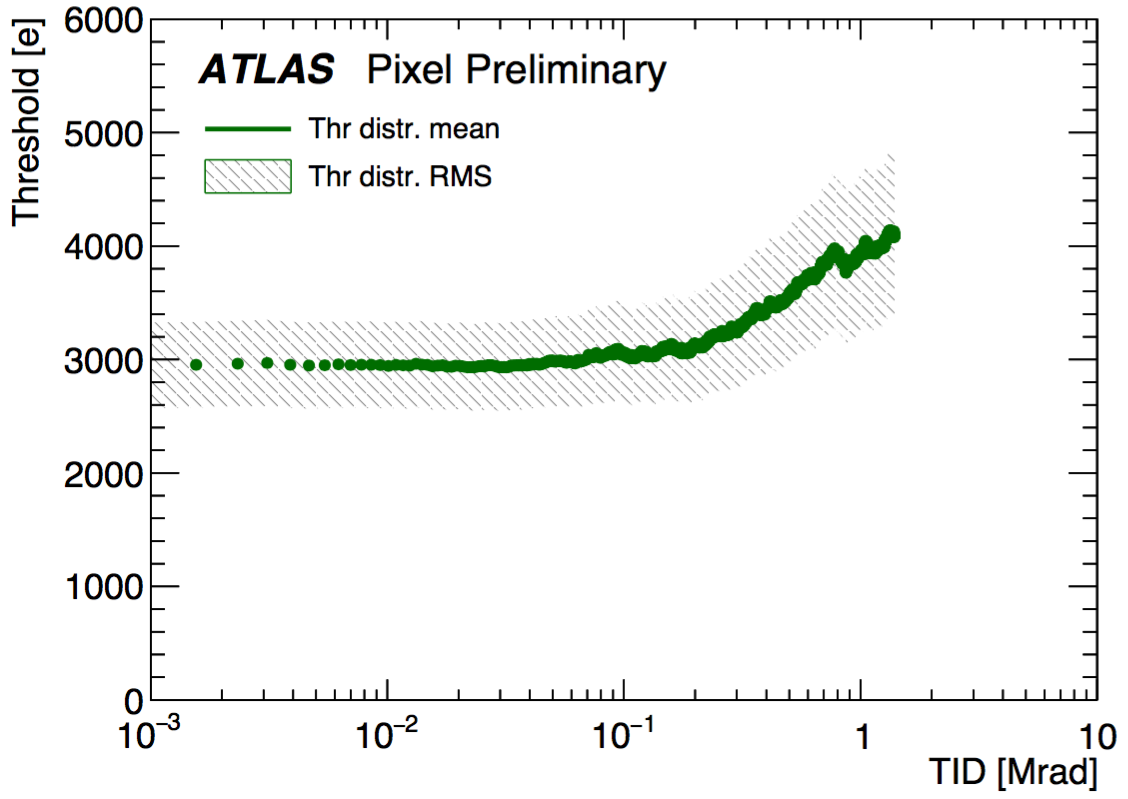
\includegraphics[keepaspectratio, scale=0.18]{tidthr.png}
  \end{minipage}
  \begin{minipage}[b]{0.5\linewidth}
    \centering
    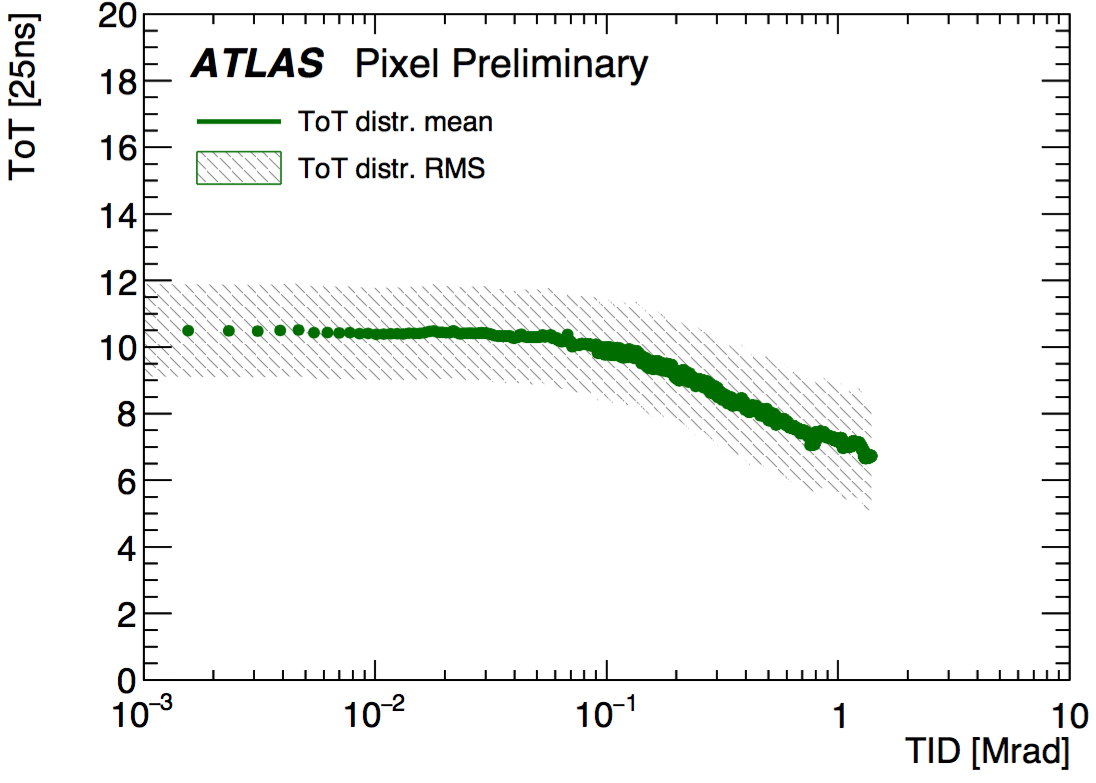
\includegraphics[keepaspectratio, scale=0.18]{tidtot.png}
  \end{minipage}
  \caption[トータルドーズ効果とThresholdおよびToTの関係]{トータルドーズ効果とThresholdおよびToTの関係 \cite{tid}。測定環境は、FEチップの周囲温度$5\ \si{\degreeCelsius}$および単位時間あたりの放射線量$10\ \si{krad}$であり、これは2016年におけるIBLの運用状況と同程度である。}
  \label{fig:tidhennka}
\end{figure}




%%------------------------------------------------------------------------------------------------------------------------
%\section{ピクセル検出器}
%\label{sec:pixelkenshutuki}
%%------------------------------------------------------------------------------------------------------------------------
%
%\fref{fig:pikuserukennshutuki}にピクセルモジュールの模式図を示す。ピクセルモジュールはシリコンセンサー、FE(\textbf{F}ront-\textbf{e}nd)チップ、フレキシブル基板から構成される。この節ではそれぞれについて説明する。
%
%\begin{figure}[tbp]
%  \centering
%  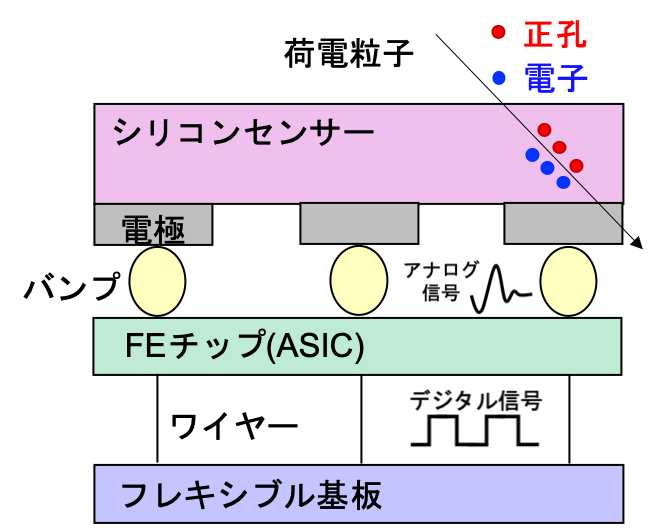
\includegraphics[height=7cm,keepaspectratio]{pikuserukennshutuki.png}
%  \caption[ピクセルモジュールの模式図]{ピクセルモジュールの模式図。}
%  \label{fig:pikuserukennshutuki}
%\end{figure}
%
%%------------------------------------------------------------------------------------------------------------------------
%\subsection{シリコンセンサー}
%\label{sec:silicon}
%%------------------------------------------------------------------------------------------------------------------------
%ATLASピクセル検出器に実装するセンサーはプラナーセンサーと3Dセンサーがある。\fref{fig:3dplanar}にプラナーセンサーと3センサーの模式図を示す。
%
%プラナーセンサーは、\fref{fig:3dplanar}の左のようにセンサーのバルク部の表面にn$^+$型半導体と$p^+$型半導体を埋め込んだ構造をしている。$n^+$型半導体電極はセンサー面において格子状に配列し、それぞれの電極から独立した信号を読み出すことができる。IBLおよびピクセル検出器ではバルク部にn型半導体を用いた、n$^{+}$-in-n型と呼ばれるものを用いている。n$^{+}$-in-n型の場合、空乏層はp$^{+}$型インプラントとn型バルクの境界から成長する。そのため、荷電粒子が空乏層を通過した際に信号をn$^{+}$電極において検知するためには、空乏領域をn$^{+}$電極まで広げる必要があり、完全空乏化しなければならない。さらに、バルク部のn型半導体は放射線損傷によりp型に型変換を起こし、空乏化の挙動が変化する。HL-LHCでは放射線損傷の影響がより大きくなることが想定されているため、センサーの挙動変化をさせないために、ITkではn$^{+}$-in-p型のセンサーを用いる。n$^{+}$-in-p型の場合、空乏領域がn$^{+}$電極とp型バルクの境界から空乏領域が成長するため、完全空乏化しなくても荷電粒子の通過により生じる電子を検知することができる。p型半導体は放射線損傷により完全空乏化電圧が大きくなるためより大きな電圧が必要になるが、全空乏化電圧が耐電圧を超えたら部分空乏化による運用が可能である。
%
%
%3Dセンサーはセンサー面に対して垂直に柱状の電極インプラントをしたものである。3Dセンサーは電極間の距離が短いことから、全空乏化に必要な電圧が小さい。さらに生成した電子正孔対が電極に到達するまでの距離も短いため、格子欠損により生じたホールにトラップされる確率もプラナーセンサーに比べて小さい。そのため、3Dセンサーはプラナーセンサーに比べて放射線耐性の高いセンサーである。3Dセンサーは放射線損傷の影響が大きいIBLの一部のみに実装されており、ITkの一部にも搭載する予定である。
%
%\begin{figure}[tbp]
%  \begin{minipage}[b]{0.45\linewidth}
%    \centering
%    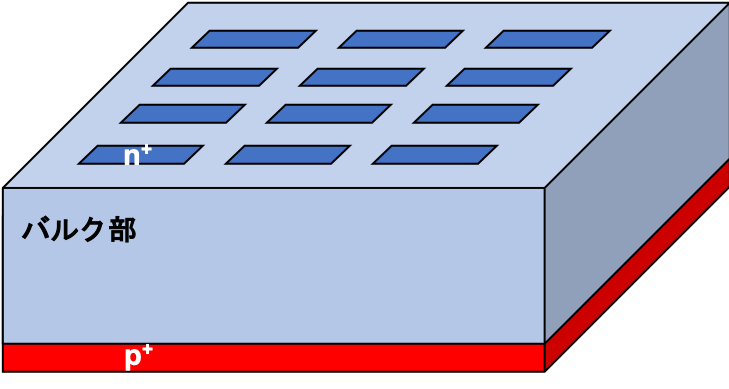
\includegraphics[keepaspectratio, scale=0.5]{planar.png}
%  \end{minipage}
%  \begin{minipage}[b]{0.45\linewidth}
%    \centering
%    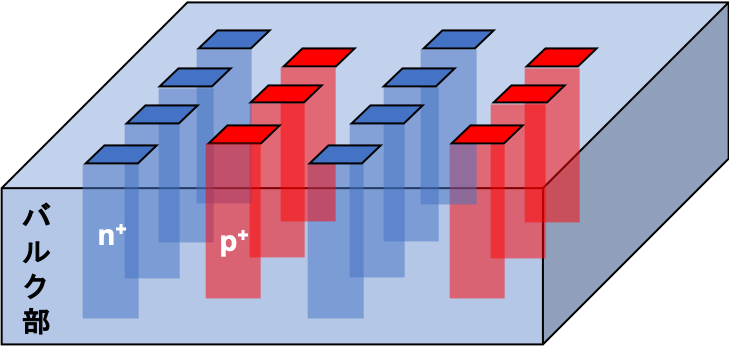
\includegraphics[keepaspectratio, scale=0.55]{3dsensor.png}
%  \end{minipage}
%  \caption[プラナーセンサーと3Dセンサーの構造]{プラナーセンサー(左図)と3Dセンサーの構造(右図)。}
%  \label{fig:3dplanar}
%\end{figure}
%
%
%%------------------------------------------------------------------------------------------------------------------------
%\subsection{FEチップ}
%\label{sec:ASIC}
%%------------------------------------------------------------------------------------------------------------------------
%
%FEチップは特定用途向けに複数機能を実装した集積回路(ASIC: \textbf{A}pplication \textbf{S}pecific \textbf{I}ntegrated \textbf{C}ircuit)である。センサーの電極で収集された電荷は、バンプを通ってFEチップに送られる。FEチップでは受け取ったアナログ信号を増幅、整形、デジタル処理を行い後段の読み出し基板に信号を送る。
%%\begin{figure}[tbp]
%%  \centering
%%  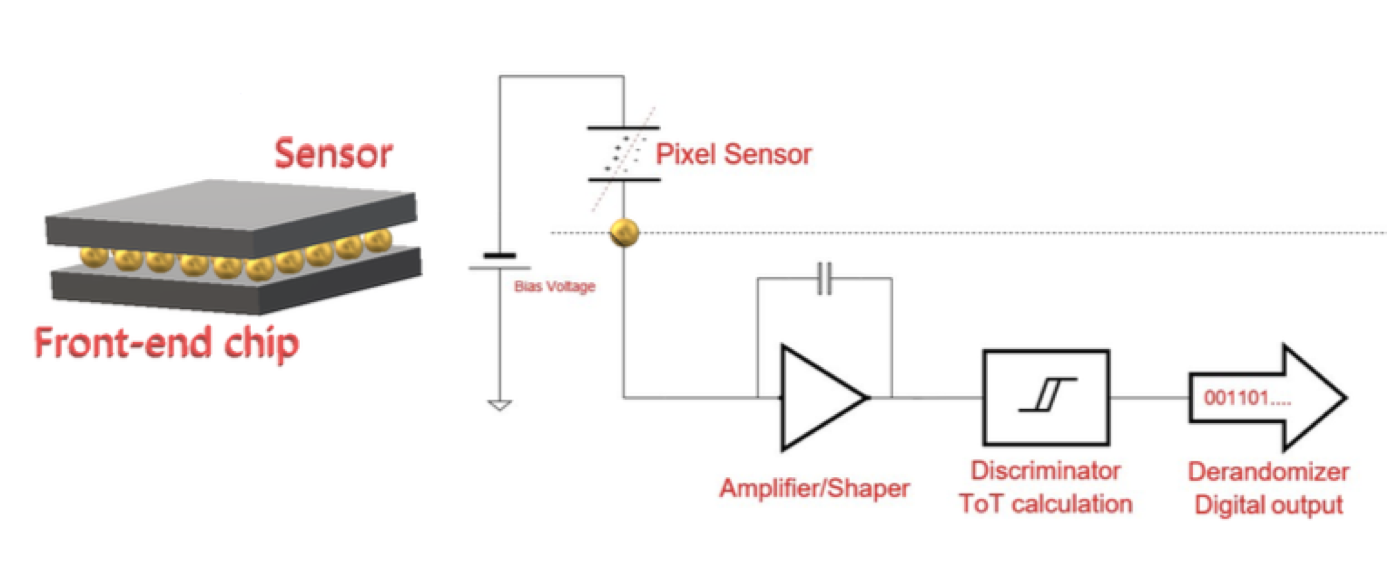
\includegraphics[height=6cm,keepaspectratio]{asic.png}
%%  \caption[シリコンセンサーの模式図]{シリコンセンサーの模式図。}
%%  \label{fig:asic}
%%\end{figure}
%
%センサーを通過する荷電粒子は、電子正孔対を生成する。シリコンの空乏層で1組の電子正孔対を生成するのに必要なエネルギーは$3.6\ \si{eV}$と一定のため、生成される電子正孔対の数はエネルギー損失$dE/dx$に比例する。
%生成されたキャリアが電極付近に収集され、電極の内部電位に影響を与えて電流が流れる。この電流から得られるアナログ信号をFEチップにおいて増幅、整形を行う。アナログ信号はアンプ回路により増幅され、三角波になるよう波形整形が行われる。信号処理されたアナログ信号がThresholdを超えた時間幅を測定し、デジタル信号に変換する。このデジタル信号を\textbf{Time over Threshold} (\textbf{ToT})と呼ぶ。アナログ信号をToTに変換する概念図を\fref{fig:tot}に示す。時間幅は$25\ \si{ns}$間隔のクロックの数で取得するため、デジタル信号として取得することができ、この信号が後段のフレキシブル基板へ転送される。
%
%\begin{figure}[tbp]
%  \centering
%  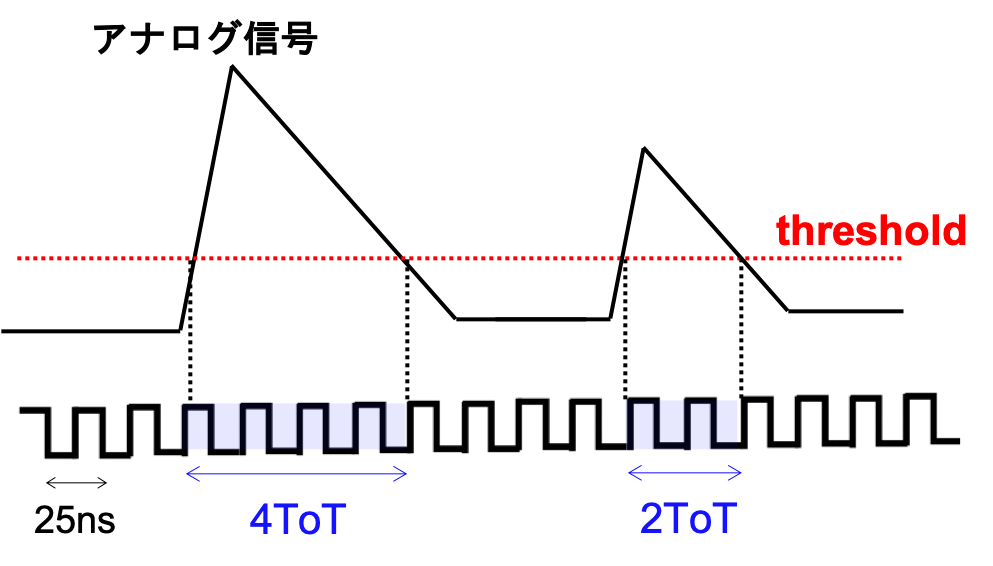
\includegraphics[height=5cm,keepaspectratio]{tot.png}
%  \caption[アナログ信号をToTに変換する概念図]{アナログ信号をToTに変換する概念図。アナログ信号の三角波はThresholdを超えた時間幅に相当する量であるToTに変換される。}
%  \label{fig:tot}
%\end{figure}
%
%また、クロックの間隔が$25\ \si{ns}$と短いため、アナログ信号のパルスの立ち上がりからThresholdを超えるまでの時間である\textbf{タイムウォーク}の効果を考慮する必要がある。電荷量とタイムウォークの関係を\fref{fig:timewalk}に示す。電荷量の小さい信号は、タイムウォークの影響が大きくなり、本来とは異なる位置からToTの測定を開始してしまう恐れがある。ATLASにおける陽子衝突は$40\ \si{MHz}$で起きているため、タイムウォークの影響が大きくなるものは異なる物理事象と関連付けてしまう可能性がある。そこで、このような影響を抑えるために、\textbf{Intime threshold}という新たな閾値を導入する。Intime thresholdはタイムウォークが$25\ \si{ns}$になるアナログ信号の波高として定義される。そのため、Intime thresholdはThresholdよりも大きい値になるよう決定され、タイムウォークの影響の制御をすることができる。
%
%\begin{figure}[tbp]
%  \centering
%  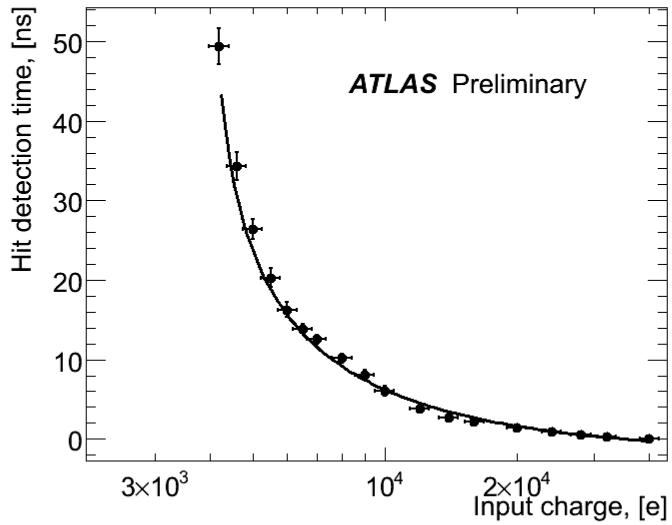
\includegraphics[height=6cm,keepaspectratio]{timewalk.png}
%  \caption[電荷量とタイムウォークの関係]{電荷量とタイムウォークの関係 \cite{timewalk}。}
%  \label{fig:timewalk}
%\end{figure}
%
%
%ピクセル検出器では\textbf{FE-I3}というFEチップを用いている。さらに読み出し速度等の性能を向上させたものが、IBLに用いられている\textbf{FE-I4}である。また、HL-LHCアップグレードに向けて新たなFEチップの開発が進んでいる。ITkに搭載する新型FEチップはITk pix v2と呼ばれており、プロトタイプであるRD53AおよびITk pix v1の製作が進んでいる。
%それぞれのFEチップの主な仕様の比較を\tref{tab:asicsiyou}に示す。
%
%\begin{table}[tbp]
%  \begin{center}
%    \caption[各FEチップの主な仕様]{各FEチップの主な仕様 \cite{itk}。}
%    \label{tab:asicsiyou}
%    \begin{tabular}{|c||c|c|c|}
%    \hline
%      項目 & FE-I3 & FE-I4 & ITk pix v2 \\
%    \bhline{1.5pt}
%      チップサイズ$[\si{mm^2}]$ & $7.6\times10.8$ & $20.2\times 19.0$ & $20.0\times 20.0$ \\
%    \hline
%      ピクセルサイズ$[\si{\micro m^2}]$ & $50\times 400$ & $50\times 250$ & $50\times 50$ \\
%    \hline
%      ピクセル数 & $18\times160$ & $80\times336$ & $400\times 384$ \\
%    \hline
%      データ転送速度$[\si{Mbps}]$ & $40$ & $160$ & $1280\times 4$ \\
%    \hline
%      トリガーレート$[\si{kHz}]$ & $100$ & $300$ & $1000$ \\
%    \hline
%    \end{tabular}
%  \end{center}
%\end{table}
%
%RD53AはATLASおよびCMS\footnote{CMSはLHC上の4つの衝突点の1つで行われている実験である。}が共同で開発を進めているHL-LHCのための試作器であり、試験・比較のために3種類のアナログ回路を搭載している。\fref{fig:rd53a}にRD53Aのを示す。\fref{fig:rd53a}のようにRD53Aには3つの領域があり、左から順にSynchronous FE、Linear FE、Differrential FEと呼ぶ。それぞれの領域においてアナログ信号の処理方法が異なり、Differential FEは他のFEと比較して電気ノイズが低くなることがわかっている。そのため、ITkにはDifferential FEを用いることが決定している。
%
%\begin{figure}[tbp]
%  \centering
%  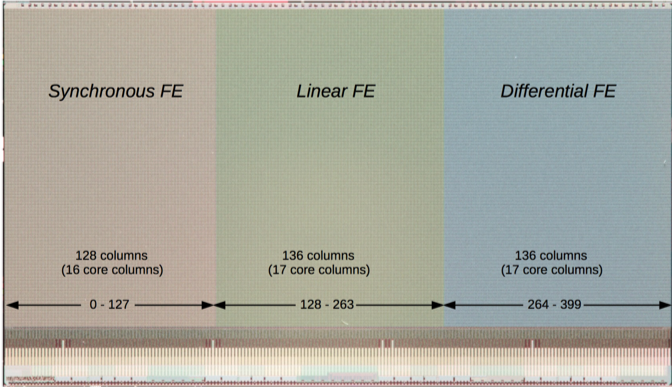
\includegraphics[height=5cm,keepaspectratio]{rd53a.png}
%  \caption[RD53Aのピクセルとアナログ回路]{RD53Aのピクセルとアナログ回路\cite{rd53a}。左の領域から順にSynchronous FE、Linear FE、Differrential FEとなっている。}
%  \label{fig:rd53a}
%\end{figure}
%
%ITk pix v1は、外形形状と主な仕様についてITkに搭載されるFEチップと同様の構造を持つ試作器である。ITk pix v1の段階で発見された不具合やバグ等を修正し量産するものが、ITkに搭載するFEチップの\textbf{ITk pix v2}である。

%To operate the chip with the sensor and to avoid problems, which results of high leakage current such as thermal runawy and additional noise, irradiated detectors are cooled down below 0°C.


%%------------------------------------------------------------------------------------------------------------------------
%\subsection{フレキシブル基板}
%\label{sec:flex}
%%------------------------------------------------------------------------------------------------------------------------
%
%フレキシブル基板はセンサーの裏側(\fref{fig:bare}の上面)に接着、およびワイヤー配線によりFEチップと電気的に接続される。フレキシブル基板の全体図を\fref{fig:flex}に示す。フレキシブル基板は、以下の3つの役割を持つ。
%
%\begin{figure}[tbp]
%  \centering
%  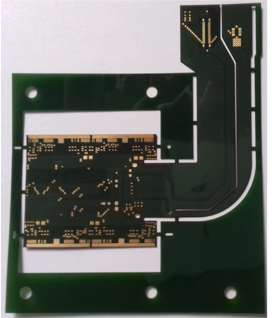
\includegraphics[height=6cm,keepaspectratio]{flex.png}
%  \caption[フレックス基板]{フレックス基板の全体図\ \cite{itk}。}
%  \label{fig:flex}
%\end{figure}
%
%フレキシブル基板は、以下の3つの役割を持つ。
%\begin{itemize}
%  \item FEチップからの信号輸送  \\
%  センサーから得られた信号はFEチップで増幅・整形され、フレキシブル基板に送られてくる。フレキシブル基板は送られてきた信号を後段のPCへ送る。
%  \item 電源の供給 \\
%  外部からの電源を、センサーとFEチップに供給する。センサーには、空乏領域を増加させるために$100\ \si{V}$程度のHV(\textbf{H}igh \textbf{V}oltage)をかける。FEチップには、電源供給のために$5.6\ \si{V}$程度のLV(\textbf{L}ow \textbf{V}oltage)
%  \item モジュールの制御システム(DCS: \textbf{D}etector \textbf{C}ontrol \textbf{S}ystem) \\
%  モジュールの温度測定のために2つのNTC(\textbf{N}egative \textbf{T}emperature \textbf{C}oefficient)が配置されている。
%\end{itemize}



%%------------------------------------------------------------------------------------------------------------------------
%\subsubsection{FE-I3}
%%------------------------------------------------------------------------------------------------------------------------
%
%%------------------------------------------------------------------------------------------------------------------------
%\subsubsection{FE-I4}
%%------------------------------------------------------------------------------------------------------------------------



%%------------------------------------------------------------------------------------------------------------------------
%\subsubsection{RD53A}
%%------------------------------------------------------------------------------------------------------------------------
%
%%------------------------------------------------------------------------------------------------------------------------
%\subsubsection{ITk Pix}
%%------------------------------------------------------------------------------------------------------------------------



\newpage
